\chapter{The consequences of a thermal shield}\label{cha:the-shield}
The primary goal of the Faraday shield is to enable particle separations closer than what would be possible without the shield, thereby enhancing gravitational interaction and reducing the required coherence times.
To reach separations $L \lesssim 100\si{\mu m}$, mutual Casimir interactions between the particles have to be shielded, as discussed in \cref{sec:2:experimental-problems}.
Until now, the shield's dynamics and properties have been ignored. However, at non-zero temperatures, thermal vibrations of the shield could significantly affect entanglement generation.
In this chapter, an estimation of the required shield size is given followed by examining the impact of thermal vibrations for both large and small shields on entanglement generation.
In the experiment, the trapped particles are cooled to their motional ground state to enable effective quantum control and the generation of spatial superpositions.
Liquid helium at $T \approx 4\si{K}$ is commonly used for cooling but cryogenic dilution refrigerators can cool small setups down to temperatures as low as $T \approx 20\si{mK}$ \cite{Zu_2022}.
These temperatures serve as reference points for all relevant calculations.


\section{Thickness and size of the shield}\label{sec:5:shield-size}
The thickness $d$ and the radius $r_s$ of the spherical shield can be estimated by considering the properties of a physical conductive material with high electrical conductivity $\sigma$.
Even a superconducting shield could be considered for an almost perfect shielding of electromagnetic fields.
The transmission $T$ of electromagnetic waves through a physical shield is given by \cite{Vandenbosch_2022}
\begin{equation}
  T = \abs{\frac{\vec{E}_\mathrm{after}}{\vec{E}_\mathrm{before}}} = \frac{2}{Z_0 \sigma d}
\end{equation}
where $Z_0 = 377\si{\Omega}$ is the impedance of free space (assuming the shield is placed in a vacuum or in air).
The electric conductivity $\sigma$ is highly dependent on the temperature \cite[p. 284-286]{Gross_2018}, decreasing approximately with $1/T^5$ at low temperatures \footnote{This behavior is valid for temperatures below the Debye temperature ($\Theta_D = 343\si{K}$ for copper). At the low temperatures used in the experiment, this model accurately describes the conductivity of metals \cite{Berman_1952}.}.
Copper offers a strong electric conductivity of $\sigma = 59.6\times 10^6 \si{S/m}$ at room temperature and measured data showing even $\sigma(T = 10\si{K}) \approx 1.5\times 10^{10}\si{S/m}$ at $10\si{K}$ \cite{Berman_1952}.

To estimate the shield's thickness, the primary criterion used, is that gravitational interactions should dominate the entanglement generation.
Other mutual interactions between the particles, such as Coulomb or Casimir forces, must be sufficiently suppressed by the shield.
The \emph{entanglement rate} $\Gamma$ quantifies the build-up of entanglement over time
\begin{equation}\label{eq:5:entanglement-rate}
  \Gamma = \dv{t} E_N(\rho)\Big|_{t=0} \, ,
\end{equation} 
where $E_N$ is an appropriate entanglement measure - in this case the logarithmic negativity \cite{Plenio_2005} introduced in \cref{sec:2:entanglement-measures}.
For gravitational interactions, the entanglement rate in the parallel orientation is given by using eq. \eqref{eq:2:entanglement-dynamics-parallel} as
\begin{equation}\label{eq:5:entanglement-rate-gravity}
  \Gamma_\mathrm{Gravity} = \frac{G M_A M_B \Delta x_A \Delta x_B}{16 \hbar L^3 \log 2} = \frac{G \pi^2 R^6 \rho_\mathrm{Silica}^2 (\Delta x)^2}{9 \hbar L^3 \log 2} .
\end{equation}
where in the last step $M_A = M_B = 4/3 \pi R^3 \rho_\mathrm{Silica}$ and $\Delta x_A = \Delta x_B \equiv \Delta x$ was used.
The entanglement rate for non-gravitational interactions, such as Coulomb or Casimir forces, must be significantly smaller than the gravitational entanglement rate, ideally by a factor $\chi > 1$.
This ensures that the measured entanglement is primarily due to gravitational interactions.
In the following sections, estimations about the thickness and size of the shield are made, to effectively screen Coulomb and Casimir forces.


\subsection{Shielding Coulomb-Interactions}
The primary role of the Faraday shield is to block electromagnetic interactions between particles.
Experimentally, it may be beneficial for the particles to carry a small amount of charge, enabling the use of electrostatic traps with high trapping strength and large controllability \cite{GonzalezBallestero_2021}. 
The Coulomb interaction potential between two charged particles is given by
\begin{equation}
  V = \frac{1}{4\pi\varepsilon_0} \frac{q_A q_B}{2L}
\end{equation}
where $\varepsilon_0 = 8.8542\times 10^{-12}\si{A^2 s^4 m^{-3} kg^{-1}}$ is the permittivity of free space and $\abs{q_{A(B)}} = e = 1.6022\times 10^{-19}\si{C}$ the charge of particle $A$ and $B$ respectively.
This interaction mimics the form of the gravitational potential and can similarly induce entanglement with a entanglement rate
\begin{equation}\label{eq:5:entanglement-rate-coulomb}
  \Gamma_\mathrm{Coulomb} = \frac{T \abs{q_A q_B} (\Delta x)^2}{64 \pi \varepsilon_0 \hbar L^3 \log 2} .
\end{equation}
The shield suppresses the coupling by a factor of $T$.
Requiring $\Gamma_\mathrm{Gravity} > \chi \Gamma_\mathrm{Coulomb}$, the minimum thickness of the shield can be calculated as
\begin{align}\label{eq:5:coulomb-gravity-condition}
  T \frac{\abs{q_A q_B}}{64 \pi \varepsilon_0} \chi \, &< \, \frac{G \pi^2 R^6 \rho_\mathrm{Silica}^2}{9} \\
  \Longleftrightarrow \quad\quad\quad\quad d \, &> \, \frac{9}{32}\frac{1}{Z_0 \sigma} \frac{1}{\pi^3 \varepsilon_0 G \rho_\mathrm{Silica}^2} \frac{e^2}{R^6} \chi .
\end{align}
The thickness strongly depends on the particles size $R$, and large or heavy particles will favor gravitational entanglement generation.
Assuming the particles are silica nano-spheres with parameters given in \cref{tab:paramters}, a minimum shield-thickness of $d \approx 10\si{nm}\chi$ at $4\si{K}$ and of $d \approx 2.5\si{\mu m}\chi$ at room temperature is required.
At low temperatures, a realistic shield thickness could therefore be $d=100\si{nm}$, balancing engineering practicality and electromagnetic suppression.
Exact estimations however depend on the realization of the experiment as well as the precision in which the evolved state is measurable.

Electrostatic fields still can propagate around the finite-sized Faraday shield and potentially induce entanglement.
It is possible to estimate the required shield radius $r_s$ to block a specific amount $\eta$ of the electric field (see \cref{apx:blocking-of-the-shield}):
\begin{equation}\label{eq:5:shield-effectiveness}
  \frac{r_s}{L} = \sqrt{\frac{1-(1-\eta)^2}{(1-\eta)^2}}
\end{equation}
The results are visualized in \cref{fig:5:shield-radius}.
\begin{figure}[!ht]
  \centering
  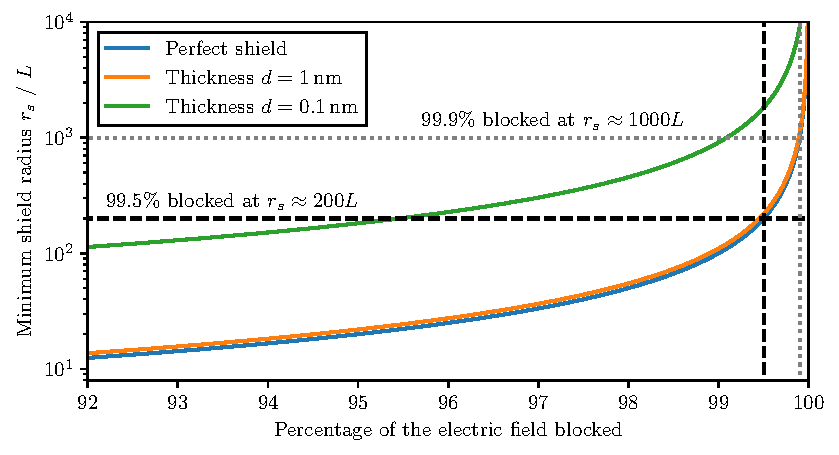
\includegraphics[width=\textwidth]{./../figures/others/shield-radius.pdf}
  \caption{Shield radius as a function of the shielding effectiveness $\eta$ for an ideal shield. Additionally, a real shield with varying thicknesses $d$ is considered at $T=300\si{K}$.
  To achieve shielding of $99.5-99.9\%$ ($\eta = 0.995-0.999$), a radius of $r_s =200-1000L$ is needed.}
  \label{fig:5:shield-radius}
\end{figure}
The shield's transmission $T$ should therefore be modified to $\tilde{T} = T\eta + (1-\eta)$, where the shielding effectiveness $\eta$ depends on $r_s$ as given by eq. \eqref{eq:5:shield-effectiveness}.
Modifying eq. \eqref{eq:5:coulomb-gravity-condition}, a minimum effectiveness $\eta_\mathrm{min}$ for sufficient shielding of
\begin{equation}
  \eta_\mathrm{min} \approx 1 - \frac{64\pi^3 \varepsilon_0 G R^6 \rho^2_\mathrm{Silica}}{9 e^2}
\end{equation}
can be approximated.
Using again the parameters from \cref{tab:paramters}, a minimum shielding of $\eta_\mathrm{min} \gtrsim 0.99997$ and thus a radius of $r_s \gtrsim 28000 L \approx 60\si{cm}$ is required.
Such a shield is too large for all practical purposes and it might be beneficial to choose heavier masses ($\tilde{M} \sim 4 M$) to reduce the shield size to the orders of $\sim 1\si{cm}$.
Due to practicality, a shield with $r_s = 1\si{cm}$ is used in the following calculations.
Uncharged particles would eliminate the Coulomb interactions and therefore reducing the shield's size and thickness to only shield mutual Casimir interactions.




\subsection{Shielding Casimir-Interactions}
Similarly to Coulomb interactions, it is possible to to estimate the required thickness for a shield to sufficiently block Casimir interactions.
The Casimir potential between the spheres with radius $R$ separated by $2L$ is given by \cite{Emig_2007}
\begin{equation}
  V = -\frac{23 \hbar c}{4\pi \cdot 128 L^7} \left( \frac{\varepsilon_r - 1}{\varepsilon_r + 2} \right)^2 R^6 .
\end{equation}
The corresponding entanglement rate is calculated similar to before by expanding the potential in small $\Delta x$ and computing the logarithmic negativity:
\begin{equation}
  \Gamma_\mathrm{Casimir} = T^2 \frac{161}{4096} \frac{c R^6 (\Delta x)^2}{\pi L^9 \log 2}\left( \frac{\varepsilon_r - 1}{\varepsilon_r + 2}\right)^2 .
\end{equation}
The dependence on $T^2$ arises because Casimir forces are second order effects in the dipole-dipole interaction \cite{Bordag_2001}.
Requiring gravitational entanglement generation to dominate, $\Gamma_\mathrm{Gravity} > \chi \Gamma_\mathrm{Casimir}$, leads to
\begin{align}
  T^2 \frac{161 c R^6}{4096 \pi L^6} \left( \frac{\varepsilon_r - 1}{\varepsilon_r + 2}\right)^2 \chi \, &< \, \frac{G \pi^2 \rho_\mathrm{Silica}^2 R^6}{9\hbar} \\
  \Longleftrightarrow \quad\quad\quad\  d \, &> \, \sqrt{\frac{1449}{4096} \frac{c \hbar}{G \pi^3}} \frac{2}{Z_0 \sigma \rho L^3} \frac{\varepsilon_r - 1}{\varepsilon_r + 2} \sqrt{\chi} .
\end{align}
For large separations, the shield thickness can be arbitrarily low, as Casimir forces vanish and at separations of $L\gtrsim 100\si{\mu m}$, the shield might not be required at all (compare \cref{sec:2:experimental-problems}).
Assuming two identical silica nano-spheres with parameters given by \cref{tab:paramters}, the required minimum thickness is between $4\times 10^{-11}\si{m} \sqrt{\chi}$ at $4\si{K}$ and $10 \si{nm} \sqrt{\chi}$ at room temperature.
This is much thinner than what is required for shielding Coulomb interactions.
The factor $\varepsilon_r$ modifies the thickness only by up to a constant factor of $\leq 1$ and is therefore ignored for worst-case estimations.

However, very thin shields lose mechanical rigidity, leading to enhanced vibrational excitations and potential instabilities.
Vibrational frequency and thus the vibrational energy depends linearly on the shield's thickness, making thinner shields prone to large decoherence due to thermal vibrations.
A detailed analysis of these effects is provided in the subsequent section.



\subsection{Gravitational effects of the shield}\label{subsec:5:shield-gravitation}
The gravitational interaction between the masses and the shield is generally neglected because it has no significant impact on the entanglement generation between the particles.
The only potential effect is indirect entanglement mediated by the thermal oscillations of the shield, as both masses couple gravitationally to it. 
However, as shown in \cref{sec:5:thermal-entanglement}, this second-order effect is very weak and does not pose a problem, since it still represents gravitationally mediated entanglement - which is the focus of the experiment anyway.
The gravitational force between a sphere with mass $M$ and a infinitesimal mass segment $\dd m = r d \rho_\mathrm{Cu} \dd r \dd \varphi$ of the shield made of copper with density $\rho_\mathrm{Cu} = 8960\si{kg/m^3}$ at a distance $r$ from the shield's center is given by
\begin{equation}
  \dd \vec{F} = \frac{G M \dd m}{\ell} \boldsymbol{\hat{\ell}} 
  \quad \Rightarrow \quad
  \dd F_z = \frac{G M r \rho_\mathrm{Cu} d}{\ell^2} \dd r \dd \varphi \cos \theta,
\end{equation}
where $\ell^2 = r^2 + L^2$ denotes the distance between the sphere and the mass segment and $\theta = \arccos L/\ell$ is the angle between them.
The total attractive force between the mass and the shield with radius $r_s$ is therefore
\begin{equation}
  F_z = GM \rho_\mathrm{Cu} d L \int\limits_{0}^{r_s} \dd r \int\limits_{0}^{2\pi} \dd \varphi \, \frac{r}{(r^2 + L^2)^{3/2}} = 2\pi G M \rho_\mathrm{Cu} d \left(1 - \frac{L}{\sqrt{L^2 + r_s^2}}\right) .
\end{equation}
For large shields $r_s \gg L$ this is independent of the particle-shield separation $L$.
For a shield with thickness $d = 100\si{nm}$ and the usual silica particle from \cref{tab:paramters}, the attraction force is around $F_\mathrm{particle-shield} \approx 4.1\times 10^{-24} \si{N}$ which is comparable with the attraction gravitational attraction force between the two particles themselves at $F_\mathrm{particle-particle} \approx 5.0 \times 10^{-24}\si{N}$ but is much weaker than the Casimir attraction between the particle and the shield with $F_\mathrm{Casimir} \approx 1.4 \times 10^{-17} \si{N}$.
Therefore, the gravitational effect of the shield can be neglected in all practical calculations.

\section{Thermal shield vibrations}\label{sec:5:thermal-vibrations}
A spherical plate with radius $r_s$ that is fixed at the edge can vibrate in different vibrational modes labeled by the indices $(k,l)$ where $k \in [1,\infty)$ and $l \in [0, \infty)$.
The exact vibrational frequency and the mode shape can only be given in terms of the Bessel functions. In fact, one of the first occurrences of these functions can be traced back to Euler trying to solve the very similar problem of a vibrating perfectly flexible membrane \cite{Dutka_1995}.
In general, the vibrations of a plate made out of a real material with thickness $d$ can be described by the differential equation \cite[p. 490]{Rao_2019}
\begin{equation}
  D \nabla^2\nabla^2 u = -\rho d \ddot{u}
\end{equation} 
where $D$ is given by material properties like Youngs module $E$ and the poisson number $\nu$ as
\begin{equation}
  D = \frac{d^3 E}{12(1-\nu^2)} .
\end{equation}
The general solution of this differential equation can be written in terms of the Bessel functions as (derived in Ref. \cite[p. 490-495]{Rao_2019}) 
\begin{equation}
  u_{kl}(r, \theta, t) = \left[J_l(\beta_k r) - \frac{J_l(\beta_k r_s)}{I_l(\beta_k r_s)}I_l(\beta_k r)\right]\cos(l\theta+\phi_1)\sin(\omega_{kl}t+\phi_2)
\end{equation}
with
\begin{equation} \label{eq:5:vibration-frequency}
  \beta_k = \frac{\tilde{r}_k}{r_s} \quad \text{and} \quad \omega_{kl} = \frac{\tilde{r}_k^2}{r_s^2}\sqrt{\frac{D}{\rho d}} = \tilde{r}_k^2\frac{d}{r_s^2}\sqrt{\frac{E}{12\rho(1-\nu^2)}} ,
\end{equation}
where $\tilde{r}_k$ is the $k$-th solution of the equation
\begin{equation}\label{eq:5:bessel-zeros}
  J_l(\tilde{r}_k)I_{l+1}(\tilde{r}_k)+I_l(\tilde{r}_k)J_{l+1}(\tilde{r}_k) = 0 .
\end{equation}
The phases $\phi_1$ and $\phi_2$ can be determined by initial conditions and refer to the rotation of the plate as well as temporal offsets. The shape of the first few modes is shown in \cref{fig:5:vibrational-modes}.
\begin{figure}[!htbp]
  \centering
  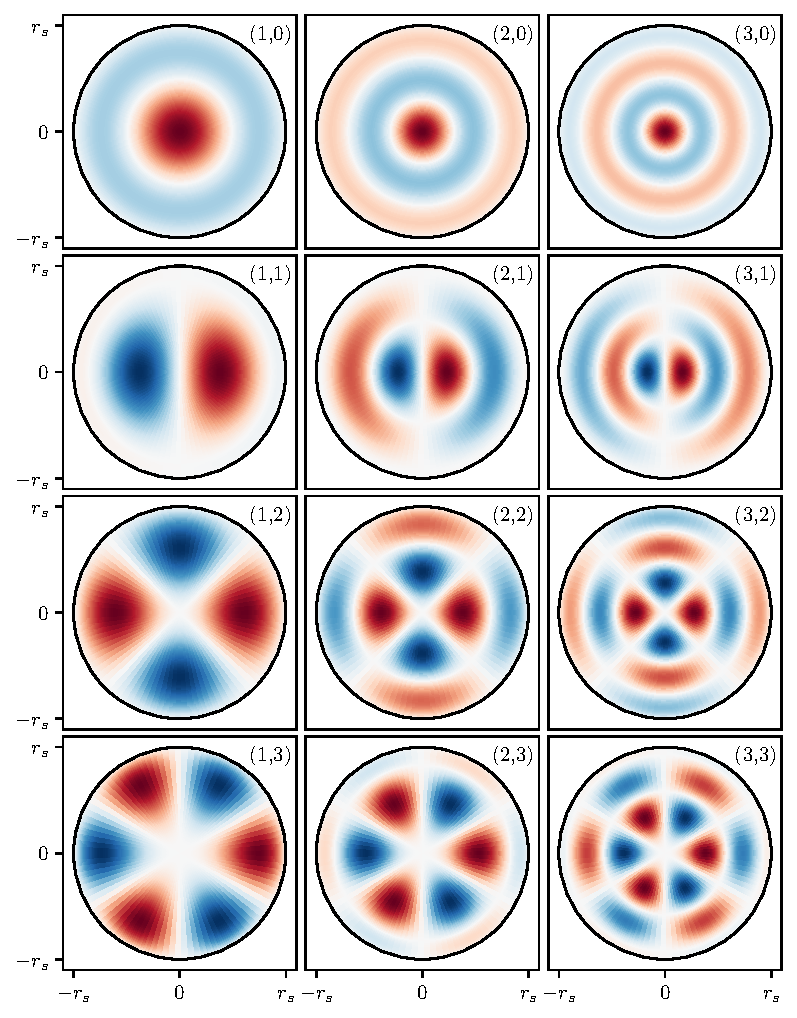
\includegraphics[width=\textwidth]{./../figures/vibrations/vibrational-modes-rd_bu.pdf}
  \caption{Shape of the first 12 modes $(k,l)$ ($k \geq 1$ and $l \geq 0$) of a vibrating spherical plate fixed at the edge with $r_s/d = 1000$.}
  \label{fig:5:vibrational-modes}
\end{figure}
In general, every possible vibration of the plates can be expressed as a sum of these default modes $u_{kl}$.
The amplitude $z$ of the vibrations are determined by the temperature $T$ and can be calculated by treating the amplitude of each vibration as a separate quantum harmonic oscillator with frequency $\omega_{kl}$.
The expectation value of the amplitude $\avg{z}$ is obviously zero and the variance $(\Delta z)^2 = \avg{z^2} - \avg{z}^2$ at temperature $T$ is given by (derivation in \cref{apx:thermal-harmonic-oscillator})
\begin{equation}\label{eq:5:amplitude-variance}
  (\Delta \op{z}_{kl})^2_T = \frac{\hbar}{2\tilde{m}\omega_{kl}}\coth(\frac{\hbar \omega_{kl}}{2k_BT}) \approx \frac{k_B T}{\tilde{m}\omega_{kl}^2} .
\end{equation}
In the last step $\hbar\omega \ll k_B T$ was used. $\tilde{m}$ is the \textit{effective mass} of the mode in which the precise shape is considered. A intuitive estimation for this mass can be given by the average amplitude of the mode 
\begin{equation}\label{eq:5:effective-mass}
  \tilde{m} = m\frac{1}{\pi r_s^2}\int\limits_0^{r_s} \dd r \int\limits_0^{2\pi} r\dd\theta \, u_{kl}(r, \theta, t)
\end{equation}
with $m=\rho \pi r_s^2 d$ being the total mass of the shield.
The amplitude of the plate vibrations are therefore in the order of $\Delta z_{kl} \propto \omega^{-1}$ at high temperatures or for low frequencies.




\subsection*{The effect of individual modes}
For a shield with radius $r_s = 1\si{cm}$ (in the following referred to as the \q{large shield}) and thickness $d=100\si{nmm}$ made out of Copper with $E = 110\si{GPa}$ and $\nu = 1/3$, the frequencies for the first few modes are between $11.0\si{s^{-1}}$ for $(1,0)$ up to $1018\si{s^{-1}}$ for like $(7,6)$.
These frequencies and thus the energy of the vibration $\hbar \omega$ is very small compared to the thermal energy $k_B T$ at all reasonable temperatures.
This means, that one expects a lot of modes to be substantially populated. Even at temperatures of $10^{-6} \si{K}$, the first $600$ modes are all equally likely to occur with a probability of $\approx 1/Z$ where $Z$ is the partition function
\begin{equation}
  Z = \sum_{m\in\{(k,l)\}} e^{-\beta \hbar \omega_m} .
\end{equation}

It is possible to calculate the asymptotic increase in the frequencies $\omega_{kl}$ for high modes $k \rightarrow \infty$.
This is, because the behavior for large inputs of the Bessel functions \cite[eq. 10.17.3]{DLMF}
\begin{equation}
  J_l(x) \sim \cos(x - \frac{l \pi}{2} - \frac{\pi}{4}) \quad \text{for} \ x \rightarrow \infty
\end{equation}
and modified Bessel functions \cite[eq. 10.40.1]{DLMF}
\begin{equation}
  I_l(x) \sim \frac{e^x}{\sqrt{2\pi x}} \quad \text{for} \ x \rightarrow \infty
\end{equation}
is known resulting in an asymptotic expansion of eq. \eqref{eq:5:bessel-zeros} 
\begin{equation}
  \sim \frac{e^x}{\sqrt{2\pi x}} \left[\cos(x - \frac{l \pi}{2} - \frac{\pi}{4}) + \cos(x - \frac{l \pi}{2} - \frac{3 \pi}{4})\right] = 0 .
\end{equation}
Therefore, the distribution of zeros $\tilde{r}_k$ is periodic for large $k$ as well as for large $l$.
The frequencies increase therefore with $\mathcal{O}(k^2 + l^2)$ for large modes.
The amplitude $\Delta z_\mathrm{kl} \propto 1/\omega$ therefore decreases quadratically with increasing mode order.
Therefore, even if at reasonable temperatures a lot of modes are occupied, the amplitude and thus the effect of each mode decreases for higher modes.
Additionally, because of the consideration of a real vibrating plate, the amplitude of the maximum of the shape $u_{kl}$ decreases for higher modes because the increased number of bulges require more material of the shield limiting the overall amplitude of the vibration even more.
Due to all these effects combined, it is sufficient to only consider the first few modes in all subsequent in numerical calculations.
However the effects of infinity many modes can be estimated asymptotically using the known scaling of $\omega_{kl}$ with increasing modes $(k,l)$.

It is also interesting to consider the scaling of the amplitudes $\Delta z$ for differently sized shields. 
According to eq. \eqref{eq:5:vibration-frequency}, the frequency $\omega$ increases quadratically with decreasing shield radius $r_s$.
However, the effective mass $\tilde{m}$ eq. \eqref{eq:5:effective-mass} depends also quadratically on the size of the shield resulting in a total dependence of $\Delta z \sim r_s$ for large temperatures and/or low modes.



% \subsection{OLDDD}


% \begin{equation}
%   \op{H} = \hbar \omega \left(\op{a}^\dagger\op{a} + \frac{1}{2}\right) + \tilde{g}_A(\op{z}) \ketbra{\psi_A} + \tilde{g}_B(\op{z}) \ketbra{\psi_B}
% \end{equation}

% Solution:
% \begin{equation}
%   \rho(t) = \frac{1}{2}\begin{pmatrix}
%     1 & e^{-i\varphi(t)}e^{-\gamma(t)}\\
%     e^{i\varphi(t)}e^{-\gamma(t)} & 1
%   \end{pmatrix}
% \end{equation}
% with the phase
% \begin{equation}
%   \varphi(t) = \frac{1}{\hbar^2\omega^2} \left(\sin(\omega t) - \omega t\right) \left(g_A^2 - g_B^2\right)
% \end{equation}
% and the decoherence term
% \begin{equation}
%   \gamma(t) = \frac{4(g_A - g_B)^2}{\hbar^2 \omega^2} \sin^2\left(\frac{\omega t}{2}\right) \left[\bar{n} + \frac{1}{2}\right]
% \end{equation}

% \begin{figure}[!htbp]
%   \centering
%   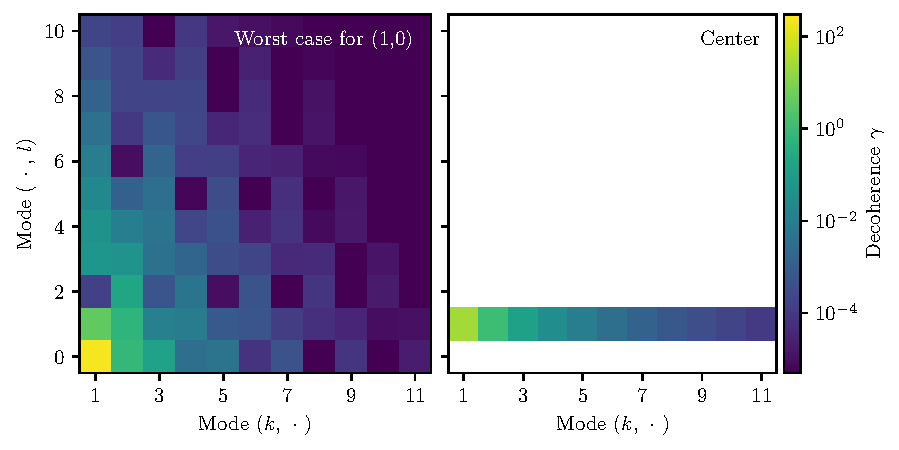
\includegraphics[width=\textwidth]{./../figures/vibrations/decoherence-analytical.pdf}
%   \caption{Maximum decoherence $\gamma$ at $4\si{K}$ for all modes if the cat-state is placed \textbf{left:} at the point with maximum gradient of the mode $(1,0)$ and \textbf{right:} in the center of the plate. It becomes evident, that only a few low modes play an actual role for the total dephasing.}
%   \label{fig:5:}
% \end{figure}


% \begin{figure}[!htbp]
%   \centering
%   \def\svgwidth{\textwidth}
%   \input{./../figures/plate-vibration.pdf_tex}
%   \caption{For a large shield, vibrations can be interpreted locally as if one mass was a distance $\Delta L$ further away from a shield and the other one $\Delta L$ closer and as if both masses would be rotated by an angle $\Delta \theta$.}
% \end{figure}

\section{Entanglement in front of a thermal shield}\label{sec:5:thermal-entanglement}
The generation of entanglement between two particles depends heavily on variations in their initial placement, as seen in \cref{cha:entanglement-generation}.
Shield vibrations can effectively be understood to alter the separation and angle of the cat-state relative to shield, as depicted in \cref{fig:5:vibrating-translation-to-variations}.
\begin{figure}[!htbp]
  \centering
  \def\svgwidth{\textwidth}
  \input{./../figures/plate-vibration.pdf_tex}
  \caption{For a large ($r_s \gg R$) and locally linearizable shield, thermal vibrations with amplitude $z$ can be interpreted as a static shield where particle $A$ (shown in red) is positioned at $L+\Delta L$ with angle $\theta$ and particle $B$ at $L-\Delta L$ with angle $-\theta$. Both variations depend solely on the vibrational amplitude. At low vibrational frequencies ($1/\omega \approx t_\mathrm{max}$), the amplitude remains nearly static during an experimental run, with thermal fluctuations distributed around $\mean{z}=0$ and variance $\Delta z$ given by eq. \eqref{eq:5:amplitude-variance}. The particles are placed at a distance $r$ away from the shield's center. Especially the cases $r=0$ and $r=0.527r_s$, where the gradient of the first mode $(1,0)$ is maximized, are considered.}
  \label{fig:5:vibrating-translation-to-variations}
\end{figure}
This approximation is only valid for shields significantly larger than the particle radius ($r_s \gg R$) and for low vibrational frequencies ($1/\omega \approx t_\mathrm{max}$), effectively capturing the impact of the first vibrational modes for small $l$ and $k$.
Especially the effect of the first mode $(1,0)$ can be put into the same framework from \cref{cha:entanglement-generation}. 
The interpretation is further supported by findings in \cref{sec:3:imperfect-plates}, showing that the Casimir interaction between a sphere and a tilted plane closely resembles that between a sphere and a flat plane.
Contrary to the problem considered in \cref{cha:entanglement-generation}, here only the thermal amplitude $z_{kl}$ is an independent random variable distributed around $\mean{z_{kl}}=0$ with a standard deviation $\Delta z_{kl}$ given by eq. \eqref{eq:5:amplitude-variance}. 
Variations in the particle-shield separation ($\Delta L$) and angle ($\theta$) are correlated to the vibration amplitude $z$.
For a large and linearizable shield, this can be understood as
\begin{equation}
  \theta = \arctan(z \abs{\nabla u}) \approx z \abs{\nabla u} \quad \text{and} \quad \Delta L = z \abs{u}
\end{equation}
where $\nabla u$ is the gradient of the vibrational mode's shape.
Performing similar calculations to those in \cref{cha:entanglement-generation}, the averaged density matrix $\mean{\rho}$, dependent on $\Delta z_{kl}$, can be derived (see \cref{apx:density-matrix-vibrating-plate}).
The resulting entanglement, quantified by logarithmic negativity as a function of temperature $T$ and particle-shield separation $L$, is given by eq. \eqref{eq:apx:en-thermal-shield} and shown in \cref{fig:5:entanglement-temperature}.
\begin{figure}[!htbp]
  \centering
  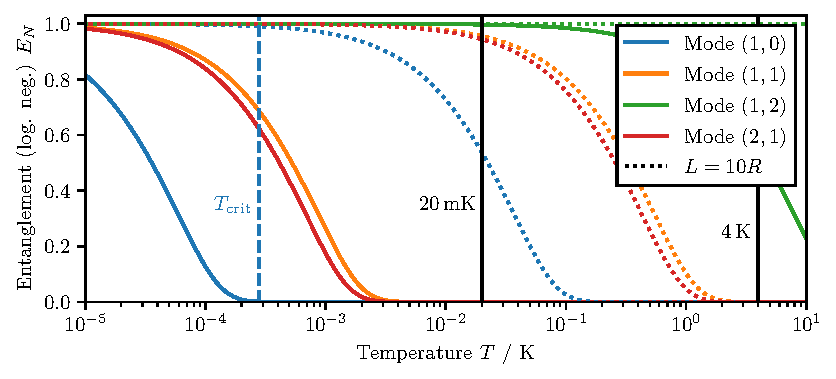
\includegraphics[width=\textwidth]{./../figures/vibrations/log-neg-shield-vibrations-T.pdf}
  \caption{Entanglement between the particles (parallel orientation) near a thermal shield at different temperatures $T$ for selected vibrational modes. At a critical temperature $T_\mathrm{crit,kl}$, entanglement is lost if mode $(k, l)$ is present. This critical point shifts with greater particle-shield separations, following $T_\mathrm{crit} \propto L^4$.}
  \label{fig:5:entanglement-temperature}
\end{figure}
At typical experimental temperatures, entanglement in the presence of the mode $(1,0)$ is observable only at large particle-shield separations.
In fact, the critical temperature $T_\mathrm{crit}$ scales with the separation $L$ in the large-separation-limit (LSL) as:
\begin{equation}
  T_\mathrm{crit} \sim (\Delta z_\mathrm{crit})^2 \sim \left(\frac{L^5}{t_\mathrm{max}} \right)^2 \sim L^4 .
\end{equation}
The large separations required are consistent with previous findings in \cref{cha:entanglement-generation}, considering that the thermal amplitudes $\Delta z_{1,0} \approx 9 \times 10^{-11}\si{m}$ at $20\si{mK}$ are comparable with the critical values the variation in the shield-particle separation $\Delta L_\mathrm{crit}$.
Interestingly, these results are unaffected by the shield radius $r_s$, as long as $r_s \gg R$ and the vibrational mode can be locally linearized.
This invariance arises because the gradient $\abs{\nabla u} \sim 1/r_s$ and $\Delta z \propto r_s$ perfectly cancel, leaving $\theta$ independent of $r_s$. 
When the cat-state orientation is parallel to the shield, the system is very stable against variations in $\Delta L$, leaving the entanglement generation completely independent of $r_s$ in first order.

However, as seen in \cref{fig:5:entanglement-temperature}, the mode number $(k, l)$ significantly impacts entanglement generation.
Higher modes correspond to higher vibrational frequencies and smaller amplitudes $\Delta z$, with $T_\mathrm{crit}$ asymptotically scaling as $\mathcal{O}((k + l)^2)$. 
This behavior is presented in \cref{fig:5:T-crit-modes}.
\begin{figure}[!htbp]
  \centering
  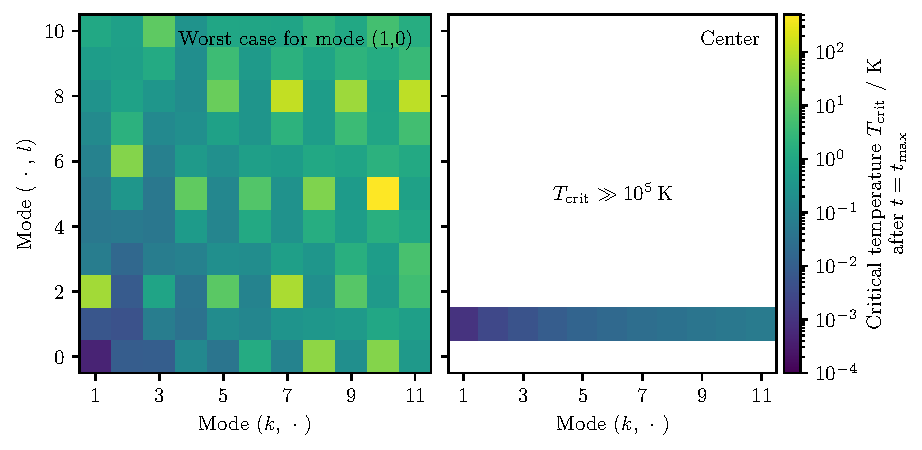
\includegraphics[width=\textwidth]{./../figures/vibrations/T-crit-modes.pdf}
  \caption{Critical temperature $T_\mathrm{crit}$, at which no entanglement is measurable anymore for different modes at a separation of $L = 2R = 2\si{\mu m}$. The shape of the vibrational modes is considered. The particle is either placed at the position of the highest gradient of mode $(1,0)$ (\textbf{left}) or in the center of the shield (\textbf{right}).}
  \label{fig:5:T-crit-modes}
\end{figure}
If the particle is positioned exactly at the center of the shield, only specific symmetric mode shapes with $l=2k+1,\ k\in\mathbb{N}_0$ can induce decoherence.
For $l > 1$, this decoherence effects become numerically negligible and are virtually indistinguishable from $0$.
If the particle is placed in the worst-case position for the first mode $(1,0)$, which corresponds to the point of maximum gradient $\abs{\nabla u}$ and thus the largest decoherence (approximately at $r \approx 0.527 r_s$), all modes are relevant.
It however becomes evident that only the first few modes significantly affect the entanglement, as higher modes do not disrupt entanglement even at temperatures much higher than those required for entanglement loss.

This naive method for calculating the decoherence induced due to the thermal shield is only accurate in the specific cases of a large and slow vibrating shield, as it requires the shield to be treaded as flat and tilted on the scale of the particle.
Furthermore, due to considering all modes separately, the combined effect is a huge overestimation, as each mode is treaded as maximally displaced simultaneously and no individual dynamics are accounted for.
In reality, the displacements of multiple simultaneously occurring modes can cancel each other partially out, reducing the overall decoherence.


\subsection{Analytic dynamics}\label{subsec:5:entanglement-analytical}
The effect of the thermal shield on entanglement generation between the two delocalized particles can be calculated analytically.
The Hamiltonian governing the interactions between the two particles with each other and with the thermal shield is given by
\begin{align}\label{eq:5:hamiltonian}
  \begin{split}
    \op{H} = &\sum_{\substack{m\in\{(k,l)\}\\ k \geq 1,\ l \geq 0}} \biggl\{ \hbar \omega_m \left(\op{a}^\dagger_m \op{a}_m + \frac{1}{2}\right) \\
    &+ g^{(1)}_\mathrm{A,m,Cas}(\op{a}_m + \op{a}^\dagger_m) \left( \ketbra{\psi^{(1)}_A} \otimes \identity \right)
     + g^{(2)}_\mathrm{A,m,Cas}(\op{a}_m + \op{a}^\dagger_m) \left( \ketbra{\psi^{(2)}_A} \otimes \identity \right) \\
    &+ g^{(1)}_\mathrm{B,m,Cas}(\op{a}_m + \op{a}^\dagger_m) \left( \identity \otimes \ketbra{\psi^{(1)}_B} \right)
     + g^{(2)}_\mathrm{B,m,Cas}(\op{a}_m + \op{a}^\dagger_m) \left( \identity \otimes \ketbra{\psi^{(2)}_B} \right)\biggr\} \\
    + g^{(1,1)}_\mathrm{Grav}&\ketbra{\psi^{(1)}_A \psi^{(1)}_B} + g^{(1,2)}_\mathrm{Grav}\ketbra{\psi^{(1)}_A \psi^{(2)}_B} \\
    + g^{(2,1)}_\mathrm{Grav}&\ketbra{\psi^{(2)}_A \psi^{(1)}_B} + g^{(2,2)}_\mathrm{Grav}\ketbra{\psi^{(2)}_A \psi^{(2)}_B}
  \end{split}
\end{align}
where the gravitational coupling
\begin{equation}
  g^{(ij)}_\mathrm{Grav} = \frac{G M^2}{L^{(ij)}}
\end{equation}
between the states $\ket{\psi^{(i)}_A}$ and $\ket{\psi^{(j)}_B}$ ($i,j = 1,2$) is determined by their separation $L^{(ij)}$ from eq. \eqref{eq:4:L-gravity}.
The shield's thermal vibrations have no influence on this coupling, hence the gravitational interaction is the same as already discussed in \cref{cha:entanglement-generation}.
Gravitational effects arising from the attraction due to the non-zero mass of the shield are omitted in these calculations because they are weaker by a factor of $10^7$ compared to the Casimir interactions, as calculated in \cref{subsec:5:shield-gravitation}.

The interaction between the state $\ket{\psi^{(i)}_{A(B)}}$ and the shield is described by the term 
\begin{equation}
  \frac{\hbar c \pi^3}{720}\left(\frac{\varepsilon_r - 1}{\varepsilon_r + 1}\right) \varphi(\varepsilon_r) \frac{R}{(\mathscr{L} + \op{z}_m u_m(r^{(i)}_{A(B)}))^2}
\end{equation}
which is dependent on the mode $m$ and the mode shape $\op{z}_m u_m$ at the position $r^{(i)}_{A(B)}$ of the cat-state in front of the shield, where $\op{z} = \sqrt{\hbar/2\tilde{m}\omega_m}(\op{a}_m + \op{a}^\dagger_m)$ is the amplitude of the vibration.
Expanding the term in first order in $\op{z}$ and ignoring the zeroth-order term, which is constant and thus equal to a global phase at the end of the calculations, the Casimir coupling in the Hamiltonian eq. \eqref{eq:5:hamiltonian} is given by
\begin{equation}
  g^{(i)}_\mathrm{A(B),m,Cas} = g_\mathrm{PFA} \frac{2 u_m(r^{(i)}_{A(B)})}{\mathscr{L}^3} \sqrt{\frac{\hbar}{2\tilde{m}\omega_m}}
  \quad \text{with} \quad 
  g_\mathrm{PFA} = \frac{\hbar c \pi^3 R}{720} \left(\frac{\varepsilon_r - 1}{\varepsilon_r + 1}\right) \varphi(\varepsilon_r) .
\end{equation} 
The combined system of the two particles $\rho_\mathrm{sys.} \in \mathcal{H}_\mathrm{sys.}$ and the thermal modes $\rho_\mathrm{th} = \bigotimes_m \rho_\mathrm{th, m} \in \mathcal{H}_\mathrm{th}$ evolves under the hamiltonian starting in the initial state $\rho_0 = \rho_\mathrm{th} \otimes \rho_\mathrm{sys.}$. 
The initial state of the two particles $\rho_\mathrm{sys.}$ is given by eq. \eqref{eq:2:initial-state} and $\rho_\mathrm{th,m}$ is the thermal state of vibrational mode $m$, which can be represented either in the number basis $\{\ket{n}\}$ or in the coherent state basis $\{\ket{\alpha}\}$ as \cite{Steiner_2024}
\begin{equation}
  \rho_\mathrm{th,m} = \frac{1}{Z} \sum_{n=1}^\infty e^{-\beta \hbar \omega_m (n + 1/2)} \ketbra{n} = \int \dd \alpha^2 \frac{1}{\pi \bar{n}} e^{-\frac{\abs{\alpha}^2}{\bar{n}}} \ketbra{\alpha} .
\end{equation} 
Here, $Z = \tr e^{-\beta \hbar \omega_m (\op{n}+1/2)} = e^{-\beta \hbar \omega_m/2}/(1-e^{-\beta \hbar \omega_m})$ is the partition function and $\bar{n} = 1/(e^{\beta \hbar \omega_m} - 1)$ is the average thermal occupation number of mode $m$ at temperature $T$. 

After time $t$, tracing out the thermal shield yields the evolved two-particle system
\begin{equation}
  \rho_\mathrm{sys.}(t) = \tr_\mathrm{th}\left(\op{U}(t) \, \rho_0 \, \op{U}^\dagger(t)\right) .
\end{equation}
The time evolution is computed in \cref{apx:thermal-shield-time-evolution} and is given by
\begin{equation}
  \rho_\mathrm{system}(t) = \frac{1}{4} \begin{pmatrix}
    1 & e^{i\phi_{11,12}} e^{-\gamma_{11,12}} & e^{i\phi_{11,21}} e^{-\gamma_{11,21}} & e^{i\phi_{11,22}} e^{-\gamma_{11,22}} \\
    & 1 & e^{i\phi_{12,21}} e^{-\gamma_{12,21}} & e^{i\phi_{12,22}} e^{-\gamma_{12,22}} \\
    \multicolumn{2}{c}{\multirow{2}{*}{c.c}} & 1 & e^{i\phi_{21,22}} e^{-\gamma_{21,22}} \\
    & & & 1 \\
  \end{pmatrix}
\end{equation}
with the decoherence terms
\begin{equation}\label{eq:5:analytical-decoherence}
  \gamma_{ii',jj'} = \sum_m \frac{4}{\hbar^2\omega_m^2} \abs{(g^{(i)}_\mathrm{A,m,Cas} + g^{(i')}_\mathrm{B,m,Cas}) - (g^{(j)}_\mathrm{A,m,Cas} + g^{(j')}_\mathrm{B,m,Cas})}^2 \sin^2\left(\frac{\omega_m t}{2}\right) \left[\bar{n} + \frac{1}{2}\right]
\end{equation}
and the phases (where the gravitational part is already given by eq. \eqref{eq:2:evolved-state})
\begin{multline}\label{eq:5:analytical-phases}
  \phi_{ii',jj'} = \sum_m \frac{1}{\hbar} \left( g^{(ii')}_\mathrm{Grav} - g^{(jj')}_\mathrm{Grav} \right) t \\
  + \frac{\sin(\omega_m t)+\omega_m t}{\hbar^2\omega_m^2}\left[(g^{(i)}_\mathrm{A,m,Cas} + g^{(i')}_\mathrm{B,m,Cas})^2 - (g^{(j)}_\mathrm{A,m,Cas} + g^{(j')}_\mathrm{B,m,Cas})^2\right] .
\end{multline}
At $T=0$, decoherence terms persist, but their effect is only significant for strong Casimir interactions (e.g., small separations $L\approx R$).
The decoherence scales as $\gamma \propto \omega_m^{-4}$ from which the asymptotic dependence on the modes $\mathcal{O}((k+l)^{-8})$ directly follows.
It is therefore possible to estimate the combined effect of the first $N$ modes as
\begin{equation}\label{eq:5:effect-of-a-mode}
  \sim \frac{1}{\zeta(8)} \sum_{n=1}^{N} \frac{1}{n^8}
\end{equation}
where $\zeta$ is the Riemann zeta function. The sum eq. \eqref{eq:5:effect-of-a-mode} converges very fast, even for small $N$.
At specific times $t=2\pi k/\omega_m, \ k\in\mathbb{N}$, the decoherence from mode $m$ vanishes, leading to entanglement values close to the ideal case, aligning with the findings in Ref. \cite{Pedernales_2022}.
This periodic behavior is confirmed in \cref{fig:5:entanglement-time-single-mode}, showing a measurable amount of entanglement only close to these specific times.
\begin{figure}[!htbp]
  \centering
  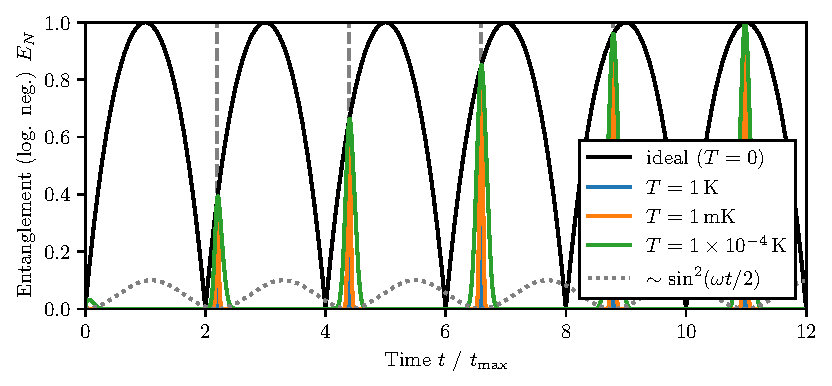
\includegraphics[width=\textwidth]{./../figures/vibrations/entanglement-hamiltonian.pdf}
  \caption{Entanglement dynamics in front of a thermal shield in mode $(1,0)$ at different temperatures. Only at specific times $2\pi k / \omega_{1,0} \approx k\times 576\si{ms},\ k\in\mathbb{N}$, entanglement is observable. This aligns with the findings in Ref. \cite{Pedernales_2022}. The particle and shield parameters are taken from \cref{tab:paramters}.}
  \label{fig:5:entanglement-time-single-mode}
\end{figure}
The full width at half maximum (FWHM) of these observed peaks is approximated by
\begin{equation}
  \mathrm{FWHM} \approx \frac{4}{\omega}\sqrt{\frac{\log 2}{\gamma}} \propto \frac{1}{\sqrt{\bar{n}}} \sim \sqrt{\omega/T},
\end{equation}
getting smaller at higher temperatures.

The resulting decoherence of multiple modes is given by the sum of all individual modes, where the contributed effect decays rapidly with the mode number, as seen in eq. \eqref{eq:5:effect-of-a-mode}.
Entanglement as seen without the shield is never reachable due to the quasi-periodicity of the system. The frequency ratios $\omega_i/\omega_j \notin \mathbb{Q}$ for $i\neq j$ \footnote{While not rigorously proven, this conclusion is supported by the transcendental nature of the zeros of the Bessel functions \cite{Lorch_1995} and the non-integer frequency ratio $\omega_{1,0} / \omega_{1,1} \notin \mathbb{Q}$, which on its own should already ensure quasi-periodic behavior.} prevent exact repetition of the resulting sinusoidal summation.
The entanglement dynamics of the first 50 vibrational modes combined are shown in \cref{fig:5:entanglement-multiple-modes} .
\begin{figure}[!htbp]
  \centering
  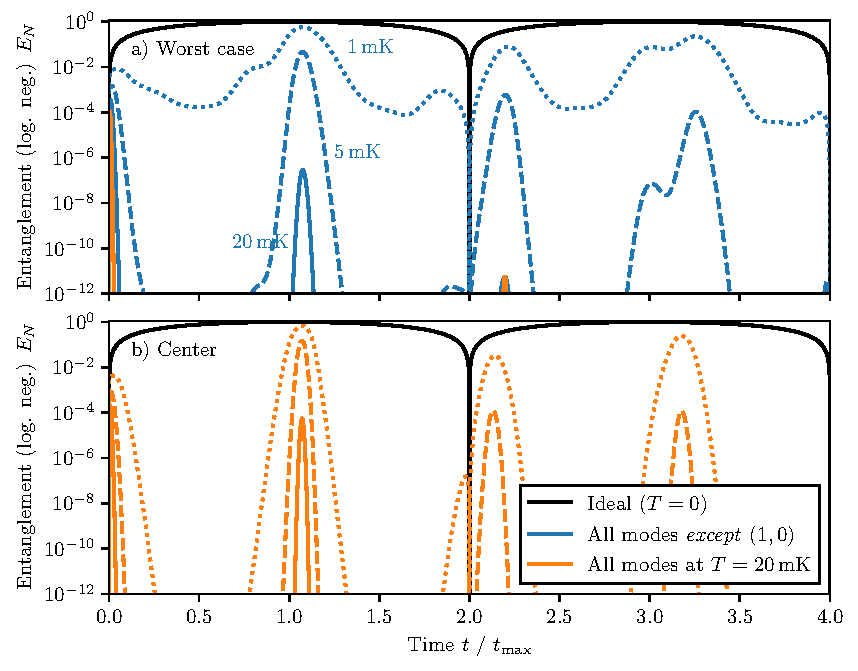
\includegraphics[width=\textwidth]{./../figures/vibrations/entanglement-dynamics-all-modes.pdf}
  \caption{Entanglement dynamics in front of a thermal shield. \textbf{Orange}: The first 50 modes have been used in the numeric calculation. The effect of all remaining modes is around $1.7 \times 10^{-11}\,\%$. \textbf{Blue}: Results excluding the $(1,0)$ mode at varying temperatures ranging from $1\si{mK}$ up to $20\si{mK}$. In part \textbf{a)} the particles are placed in the worst-case position of the shield where the effect of the mode $(1,0)$ is maximized. In \textbf{b)} the particles are placed in front of the center of the shield. The parameters used are taken from \cref{tab:paramters}.}
  \label{fig:5:entanglement-multiple-modes}
\end{figure}
This figure highlights the dominant contribution of the first mode $(1,0)$, with realistically measurable entanglement primarily occurring at $t = 2 \pi/\omega_{1,0}$.
Even for temperatures as low as $20\si{mK}$, entanglement remains minimal due to large decoherence.
Increasing the particle-shield separation reduces Casimir coupling $g_\mathrm{Cas} \propto \mathscr{L}^{-3}$ and hence reducing the decoherence while simultaneously slowing gravitational entanglement generation down ($t_\mathrm{max} \propto L^3$).
The combined effect is therefore qualitatively given by $\gamma \propto g_\mathrm{Cas}^2 \sin^2(t) \propto L^{-6} \sin^2(L^3) \xrightarrow{L \gg R} 0$, suggesting that no decoherence is present at large separations.
The dependence of entanglement on the particle-shield separation at two specific points in time is shown in \cref{fig:5:entanglement-thermal-shield-L}.
\begin{figure}[!htbp]
  \centering
  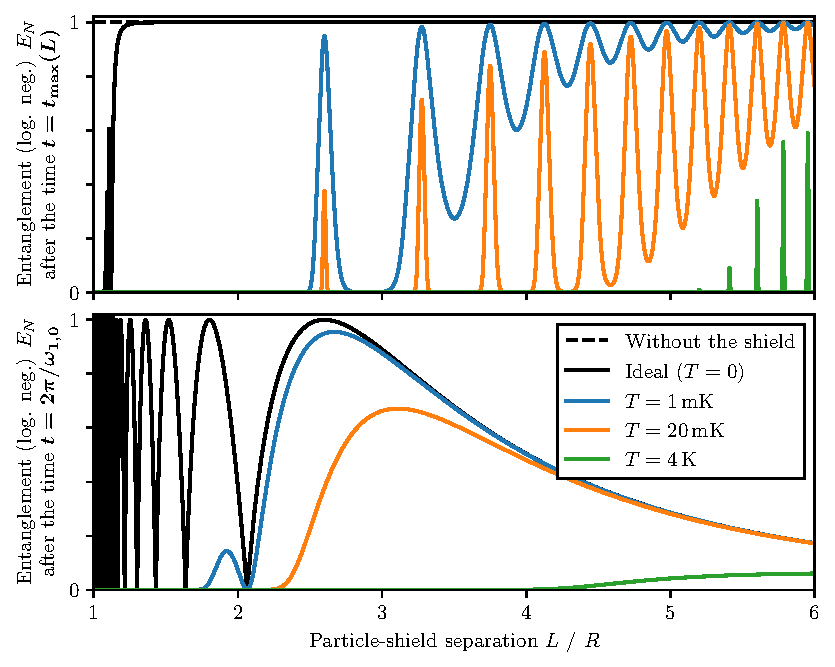
\includegraphics[width=\textwidth]{./../figures/vibrations/all-modes-entanglement-L.pdf}
  \caption{Entanglement generation for different particle-shield separations $L > R$ and different temperatures at times $t_\mathrm{max}(L)$ (eq. \eqref{eq:4:t-max}) (\textbf{top}) and $t = 2\pi/\omega_{1,0}\approx 576\si{ms}$ (\textbf{bottom}). Calculations use parameters from \cref{tab:paramters} and the particles are placed in the worts-case position in front of the shield, where the effect of the mode $(1,0)$ is maximized.}
  \label{fig:5:entanglement-thermal-shield-L}
\end{figure}

By measuring after a time $t_\mathrm{max}(L)$ (with $t_\mathrm{max}(20\si{\mu m}) \approx 258\si{ms}$), in the ideal scenario without the shield, a maximally entangled state with $E_N = 1$ is observed.
Although $2\pi/\omega_{1,0}$ is constant in time, $t_\mathrm{max}$ increases with $L$, creating specific separations (e.g. for $L\approx 2.6R$) where the two times align, enhancing observability.
For even larger $L$, decoherence effects eq. \eqref{eq:5:analytical-decoherence} diminish, making entanglement measurable even at higher temperatures.

By measuring at the time $2\pi/\omega_{1,0} \approx 576\si{ms}$ where the decoherence of the first mode almost vanishes, entanglement can be observed by increasing the particle-shield separation.
However, measuring at a constant time independent of $L$ limits the maximum of possibly reachable entanglement as the gravitational entanglement rate slows down and increasing $t_\mathrm{max}$.

The radius of the shield also has a large impact on entanglement generation. Smaller shields with larger mode frequencies result in a decreased and faster oscillating decoherence $\gamma \propto \sin^2(\omega) 1/\omega_m^2$.
The time between the points, where the decoherence effect of the first mode almost vanishes (i.e. every $\Delta t = 2\pi/\omega_{1,0} \propto r_s^2$), decreases for smaller shields and thus making entanglement measurable more frequently at almost any point in time.
Numeric calculations show, that even for shields as large as $r_s = 5\si{mm}$, entanglement of around $E_N \lesssim 1$ can be measured at $T = 20\si{mK}$ even at close separations (see \cref{fig:apx:entanglement-thermal-shield-rs-5mm} and \cref{fig:apx:entanglement-thermal-shield-rs}).

\subsubsection*{Indirect entanglement through the shield}

Examining the phases $\phi_{ii',jj'}$ in eq. \eqref{eq:5:analytical-phases} reveals that, similar to the gravitational force, the Casimir interaction between the particle and the shield can induce entanglement between the particles. This occurs as both particles couple to the shield via Casimir interactions, enabling indirect interaction between them.
However, the resulting amount of entanglement is very small, as evident from the dependence on $1/\hbar^2$ in eq. \eqref{eq:5:analytical-phases}.
While negligible at larger separations, Casimir-induced indirect entanglement could become significant at very small distances where the Casimir forces are much stronger than the gravitational interaction. 
This is particularly relevant if the entanglement generated via Casimir interactions approaches that due to gravity. 
The relative strength can be estimated by comparing the term corresponding to the gravitational interaction with the Casimir terms in eq. \eqref{eq:5:analytical-phases}:
\begin{align}
  g_\mathrm{Grav} t &\gtrsim \frac{\sin(\omega_m t) + \omega_m t}{\hbar \omega_m^2} g_\mathrm{Cas}^2 \\
  \Longrightarrow \quad 
  \frac{G M^2}{2L} &\gtrsim g_\mathrm{PFA} \frac{1}{\mathscr{L}^3} \sqrt{\frac{\hbar}{2\tilde{m}\omega_m}}
\end{align}
where $\mean{\sin(\omega t)} = 0$ was averaged.
Using the parameters for the particles and the shield from \cref{tab:paramters}, the lower bound for the separation is given by $L > 1.29\times 10^{-5}\si{m}\approx 1.3 R$. For separations $L \gtrsim 2.7R$, gravitational entanglement becomes $100$ times stronger than entanglement due to Casimir interactions.
These separation limits are most likely fulfilled either way considering the results from the previous chapters, thus indirect entanglement can be neglected in all practical circumstances.



\subsection{Small shields}
A small shield can only block the direct Casimir interactions between the particles $A$ and $B$, hence it can only be used if no other forms of electromagnetic interactions between the particles such as Coulomb coupling are present.
For very small shields in the size of the particles $r_s \sim R + \Delta x / 2$, the above considerations are not fully applicable, as they assume the linearization of the vibrational mode at the particle's scale.
The vibrations of the shield and the resulting vibrational modes substantially alter the Casimir potential, which is no longer determined solely by the interaction between a perfectly flat shield and a spherical particle. 
Deformations can no longer be approximated locally as a flat, tilted plate; instead, the shape of the vibrational mode must be accounted for. 
As discussed in \cref{sec:3:imperfect-plates}, deformations, such as those resembling the first vibrational mode, significantly impact the resulting Casimir potential which is, in the proximity-force approximation, bounded by an interaction equivalent to that between a sphere and a plate with separation $\mathscr{L} \pm \Delta z$.

In the temporal domain, vibrational frequencies scale quadratically with the shield size, $\omega \propto 1/r_s^2$, which results in the measuring process being multiple times longer than a single vibrational period. 
Consequently, Casimir interactions are averaged over time, leading to an effectively planar and flat shield.
This agrees with the findings in the previous section and the results shown in \cref{fig:apx:entanglement-thermal-shield-rs-5mm}, where smaller shields exhibit drastically reduced decoherence effects.

Similar reasoning applies to higher vibrational modes in arbitrarily large shields. 
These modes, characterized by high frequencies and a roughly uniform  distribution of deformations, effectively average out the Casimir interactions in the temporal domain as well as because of the findings in \cref{sec:3:imperfect-plates}, preserving entanglement.


\section{Discussions}\label{sec:4:discussion}
The preceding results highlight, that the proposed Faraday shield in experiments on measuring gravitationally induced entanglement entail significant engineering challenges, particularly due to the strict accuracy requirements for particle placement.
Variations must be minimized to a precision of approximately $\Delta L \simeq 10^{-10}\si{m}$ and $\Delta \theta \simeq 10^{-9}\si{rad}$, which are extremely stringent.
Even the rotation of the earth ($\omega_\mathrm{Earth}\approx 7.3\times 10^{-5}\si{rad/s}$) could potentially be problematic, because if small fluctuations in the measurement time $\Delta t \gtrsim 10^{-4}\si{s}$ are present, this corresponds to an additional angular uncertainty of $\omega_\mathrm{Earth}\Delta t \gtrsim \Delta \theta_\mathrm{crit}$.
Adjustments to the experimental parameters in \cref{tab:paramters} have to be made, where especially the separation distance $L$ and the orientation are easily changeable.

The parallel configuration is very stable against variations in the distance and might therefore be favorable (see in \cref{fig:4:optimal-orientation}).
The separation $L$ can be freely chosen and larger distances reduce the effect of placement variations as seen in \cref{fig:4:theta-crit-L}, while simultaneously increasing the required coherence time $t_\mathrm{max} \propto L^3$.

It could also be argued that at a distance of $L \geq 100\si{\mu m} = 10 R$ (compare to \cref{sec:2:experimental-problems}), the Faraday shield would no longer be required because the Casimir forces are approximately ten times weaker than gravitational interactions.
However, the loss of entanglement due to angular and distance variations is not purely due to the Casimir forces between the particle and the shield.
The gravitational coupling also depends on the placement, so that a complete removal of the shield does not fully eliminate the need for high placement accuracy.
Without the shield and by gravitational interaction alone, the critical variations are given by $\Delta \theta_\mathrm{crit,\,ideal} = 1.1 \times 10^{-3}\si{rad}$ and $\Delta L_\mathrm{crit,\,ideal} = 7\times 10^{-4}\si{m}$, which should not pose an engineering problem.

Other parameters, such as particle size and superposition size, may not be easily adjustable without increasing the complexity of quantum control.
Furthermore, particle trapping and levitation is not a limiting factor, as stable trapping is achievable for various configurations (\cref{sec:4:trapping}).

A primary aim of this thesis is to assess whether the Faraday shield allows particles to be brought closer together to enhance gravitational entanglement and reduce coherence times. 
Using the previous results, a optimal experimental parameter space can be determined.
The optimization-goal can be expressed as the following:

One wants to get \textit{as much entanglement as possible} in the \textit{shortest time possible} while allowing for the \textit{largest uncertainties} in the state preparation and considering the limitations in the particles mass as well as in the superposition size.

Without specific constraints, a general optimization is impossible because (if the mass $M$ and the superposition size $\Delta x$ is fixed) coherence time $t \propto L^3$ (eq. \eqref{eq:4:t-max}) and critical angular variation $\Delta \theta_\mathrm{crit} \propto (L-R)^3/L^3$ (for small separations) or $\Delta \theta_\mathrm{crit} \propto L^2$ (for $L \gg R$) cannot be optimized simultaneously.
With constraints such as target coherence time $t_\mathrm{target}$ and/or a minimum placement accuracy, the required sphere-plate separation $L$ as well as maximum measurable entanglement can be determined using the following steps:
\begin{enumerate}
  \item Let us assume that the size of the particle $R$ and consequently the mass $M=4/3 \pi R^3 \rho_\mathrm{Silica}$ as well as the superposition size $\Delta x$ are fixed. An increase in either of them would have a positive effect of the optimization goal stated above, as the time $t_\mathrm{max}$ decreases and the stability against placement variations increases simultaneously.
  \item Given placement accuracies in angular and separation variations determine the optimal orientation $\alpha,\beta$ of the setup as seen in \cref{fig:4:optimal-orientation}. Experimentally reachable coherence times may influence this decision slightly by taking \cref{fig:4:t-max-orientation} into account. Most likely, the most stable orientation is going to be the parallel one with $\alpha = \beta = 0$.
  \item The following ratio given by the entanglement rate eq. \eqref{eq:4:t-max}
  \begin{equation}
    \frac{M^2 (\Delta x)^2}{L^3}t_\mathrm{max} = \frac{4 \pi \hbar}{G}\abs{\sin\alpha\sin\beta-\frac{1}{2}\cos\alpha\cos\beta}^{-1} \sim 10^{-23} \si{kg^2 s/m}
  \end{equation} 
  is fixed therefore \cite{Aspelmeyer_2024}.
  \item In general it is possible to measure at an earlier time $t_\mathrm{target} = \tau t_\mathrm{max}$ (i.e. the coherence time) with $\tau \leq 1$, where less entanglement has been generated but a larger stability against placement variations can be tolerated (see \cref{fig:4:time-delta-theta}). Putting all assumptions together, the product
  \begin{equation}\label{eq:4:fixed-ratio}
    \tau L^3 = \frac{t_\mathrm{target} G M^2 (\Delta x)^2}{8\pi \hbar} = \mathrm{const.}
  \end{equation}
  of measurement time and particle-shield separation is constant.
  \item In the parallel orientation, the distance variations don't matter as the system is very stable against variations in the particle-shield separation. The critical angular variation however scales like $\Delta \theta_\mathrm{crit} \sim (L-R)^3/L^3$ for small distances and like $\Delta \theta_\mathrm{crit} \sim L^2$ at larger distances as shown in \cref{fig:4:theta-crit-L}. It is therefore possible to determine the minimum separation $L_\mathrm{min} > R$ for a given placement accuracy.
  \item Using the required separation, one can calculate $\tau \in (0, 1]$ using eq. \eqref{eq:4:fixed-ratio} and look up the maximal possible entanglement in \cref{fig:4:time-delta-theta} after an evolution time $\tau t_\mathrm{max}$.
\end{enumerate}
As an example, the radius is fixed at $R=10\si{\mu m}$ and the superposition size is $\Delta x = 100\si{nm}$. Let's say that such a particle can be placed with an accuracy of $\Delta \theta = 5 \times 10^{-8} \si{rad}$ and a coherence time of $1\si{s}$ is reachable. 
Using the steps outlined above, the required minimum particle-shield separation is around $L\approx 8R$ and the maximal amount of measurable entanglement is given by $E_N \approx 6.0\times 10^{-2}$.
For more entanglement, either a heavier particle, a larger superposition size, a higher placement accuracy or larger coherence times are required. 
It is therefore possible to bring the particles closer together than without the Faraday shield and still measure entanglement.
One is only limited by the placement accuracy and repeatability.